\chapter{Estudio de Diagnóstico}

\section{Seguimiento de la Pandemia}

A causa del COVID-19, a nivel global se han registrado aproximadamente 34 millones de personas contagiadas y 1 millón de muertes confirmadas hasta la fecha 1 de Octubre del año 2020,cuyo desenlace causa pánico y desorden público a través del mundo. La Organización Mundial de la Salud (OMS) declaró al COVID-19 como una emergencia de salud internacional, dando recomendaciones para prevenir y controlar el contagio de la misma. En Bolivia se tiene registrados 135,311 enfermos, de los cuales 7.965 han fallecido y 31.817 casos activos restantes, además de 95.529 pacientes dados de alta, dando al COVID-19 un ratio de mortalidad de 5,89\% en Bolivia. Eventualmente se tomaron medidas de prevención, las cuales son fuertemente criticadas independientemente de la calidad de resultados, siendo la principal la declaración de una cuarentena que ha impactado servicios de transporte, comercio, entretenimiento, educativo y muchos más; por lo cual se han estado viendo sofocadas las posibilidades de salir libremente y realizar actividades que solían ser consideradas como cotidianas.\\

Esta cuarentena implicó que las ciudades del mundo impongan nuevas leyes de confinamiento, implementando advertencias, multas y cárcel para quienes incumplan las mismas, así mismo, se cancelaron eventos festivos, se cerraron escuelas y pospusieron clases, incluso negocios que no eran considerados necesarios para la primera necesidad de la población tuvieron que cerrar temporalmente durante largo tiempo hasta que las personas adoptaron costumbres de higiene personal. El deporte ha sufrido especialmente debido a la influencia del COVID-19 como nunca antes ha acontecido, por ello las personas, especialmente los deportistas precisan de mantener sus rutinas diarias de ejercicio físico y las empresas deben planear nuevos modelos de negocio en orden de ajustarse a los cambios.\\

Se recomienda hacer ejercicio durante al menos 30 minutos cada día o al menos 20 minutos de exigencia vigorosa. En cuanto a niños, ancianos o enfermos crónicos, consultar con un medico es recomendado. Mantenerse en casa es efectivo para evitar la expansión de esta enfermedad, pero mantener la actividad física es un punto importante.\\

El ejercicio en casa puede realizarse de demasiadas formas y muy variadas, basta con buscar un ambiente que respete las medidas de prevención para el COVID-19 y sea un espacio mínimamente grande para moverse cómodamente con los brazos y piernas extendidos, aunque no sean de las mejores practicas, es incluso suficiente un metro cuadrado para entrenar en distintos deportes o disciplinas. Se pueden exhibir múltiples ejemplos de ejercicio, por lo que es casi imposible tener una excusa, la población que no puede darse el lujo de ejercitarse, esta en una situación deplorable económicamente, carece del tiempo debido a un exceso insano de trabajo, problemas de salud u otros.
Se pueden realizar entrenamientos desde flexiones, sentadillas, abdominales, trotar en el mismo lugar y hacer juego de pies, así mismo se puede practicar Yoga, Tai Ji Quan, Karate, Tae Kwon Do y diversas artes marciales que poseen técnicas y practicas tanto en ambientes grandes como pequeños y puede ser practicado en relativamente cualquier momento, solo con la presencia de voluntad y un tiempo bien administrado. Existen innumerables vídeos y guías de ejercicio para realizar en Internet y televisión e incluso juegos o aplicaciones para poder ejercitarse lo necesario o ir más allá.\\

Esto no significa que el deporte o el ejercicio deba ser obligatoriamente limitado o que se deben restringir si no se cumple con estas restricciones, sino que esta es una medida más en contra de la expansión del COVID-19 hasta que exista una vacuna o resistencia efectiva ante ella \cite{Chen}. \\

La tutoría de entrenadores a deportistas siempre ha sido a partir de ordenes y tutoriales cuya base teórica es el enfoque cognitivo (aprender procesando la información a partir de lo que vemos y adquirimos de esa experiencia). Esto significa que la experiencia personal y el entrenamiento previo o visualización de resultados de los entrenadores se verá reflejado en su metodología de enseñanza, señalizando principalmente ordenes de ejecución de movimiento, entrenamiento mental (cuyo objetivo es desarrollar la autoestima y pensamiento/visualización positiva) y la retroalimentación para corregir errores y perfeccionar la técnica\cite{raiola2017motor}. \\
\section{Investigación Sobre Los Dispositivos Pioneros en el área de Body Tracking}

En principio, el Body Tracking con cámaras ha ido evolucionando y existen varias herramientas y entornos que se explicaran a futuro en el Estudio de Alternativas, que permiten introducir a campos de estudio y entretenimiento a experimentar con el uso de las herramientas de Body Tracking, como el medico y educativo.\\

\subsection{Kinect desarrollado por Microsoft}

Para exponer un ejemplo revolucionario de esta nueva rama, se menciona el dispositivo Kinect, siendo uno de los dispositivos más famosos, pero desacreditado del potencial que una vez tuvo, fue desarrollado por Microsoft por 20 años, se publico el año 2010 y su venta se descontinuo en abril del 2016, debido a la llegada de nuevas alternativas como la realidad virtual, su trágica implementación al mercado que decanto a los usuarios y  su sobre coste consumaron el hecho, a pesar de ello, desde el 2011 se lo adapto para PC desde Windows 7 y permitió el desarrollo libre. \\

Una fortaleza del desarrollo de está tecnología son las opciones que enriquecen las posibilidades de los usuarios en su experiencia con la tecnología, siendo el principal beneficiario la industria de los videojuegos. 
"Kinect ofrece una increíble cantidad de diversión a jugadores casuales, y su creativo concepto de ser libre de un control es innegablemente atractivo" denota una reseña realizada por IGN. Si bien los sistemas interactivos que emplean Body Tracking son duramente criticados tanto por críticos y usuarios, no se puede dudar de su éxito en ventas, se distinguió por ser el dispositivo electrónico de consumo más vendido en el Guiness World Records durante ese año.\cite{7934445}\\
Posteriormente, al mencionar Sistemas Interactivos con Body Tracking, se requiere de denotar la dificultad de mostrar resultados, debido a la pobreza de condiciones en muchos ambientes que los usuarios tienen, subiendo las expectativas de su desarrollo. 

\begin{figure}
	\centering
	\begin{subfigure}{.5\textwidth}
		\centering
		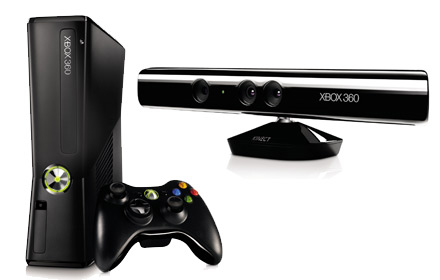
\includegraphics[width=6cm,height=3cm,]{./Images/kinectex.jpg}
		\caption{Dispositivo Kinect}
		\label{kinectex}
	\end{subfigure}%
	\begin{subfigure}{0.5\textwidth}
		\centering
		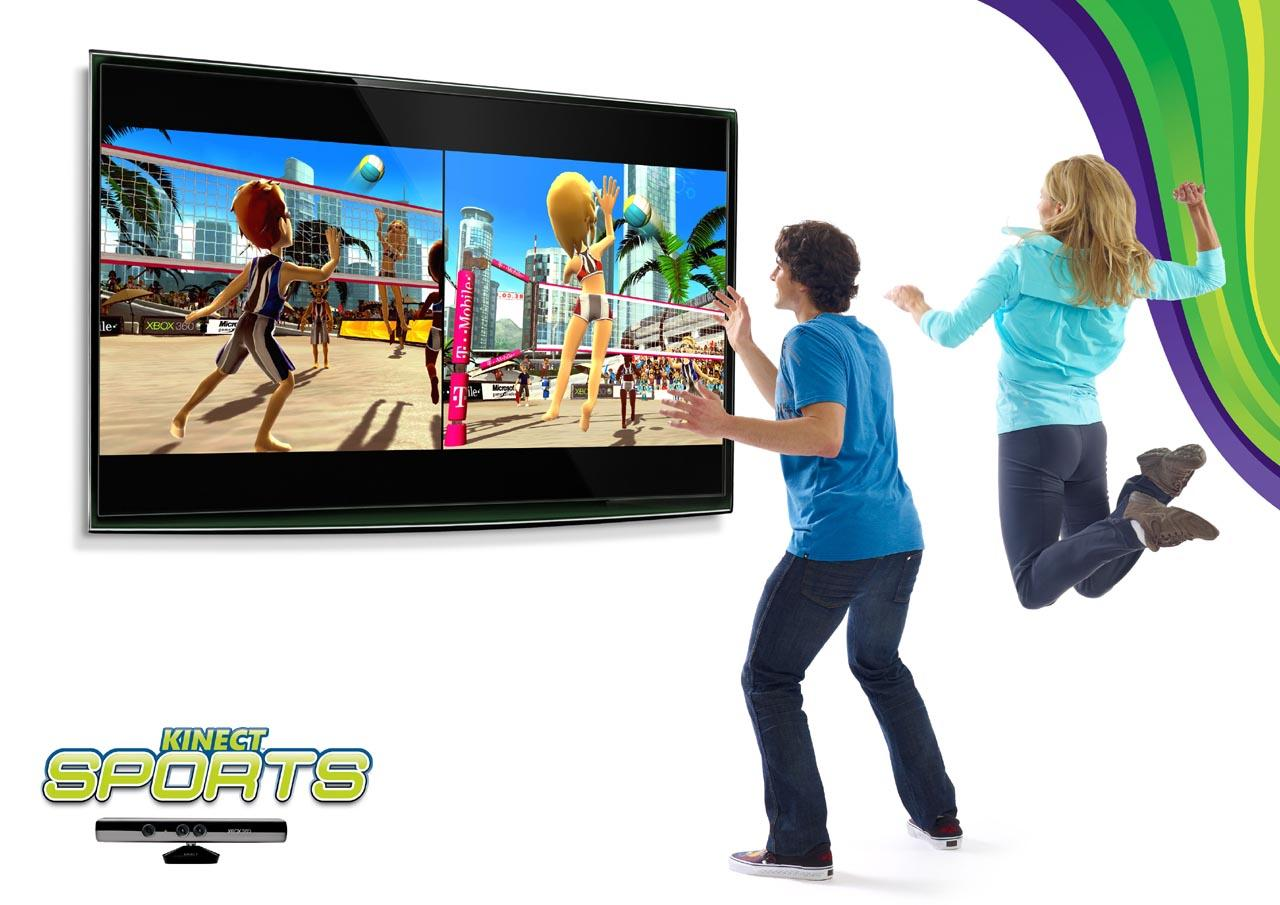
\includegraphics[width=6cm,height=4cm,]{./Images/kinectexuse.jpg}
		\caption{Ejemplo de Uso de Kinect}
		\label{kinectexuse}
	\end{subfigure}
	\caption{Ejemplo de un Kinect y su Uso en el Sistema Interactivo Kinect Sports}
	\label{kinectExample}
\end{figure}

\subsubsection{Azure Kinect}

Es una versión moderna y reciente por parte de Microsoft, consta de un sensor de profundidad con opciones de reducción del campo de visión (FOV) para optimización de la aplicación, posee un micrófono para mejorar la captura de sonido, una cámara RGB, un acelero metro, un giroscopio y permite la sincronía de lectura de múltiples dispositivos Kinect para el desarrollo de un proyecto. Sin embargo, este equipo no esta disponible, por lo que su sola mención es suficiente.

\begin{figure}[t!]
	\centering
	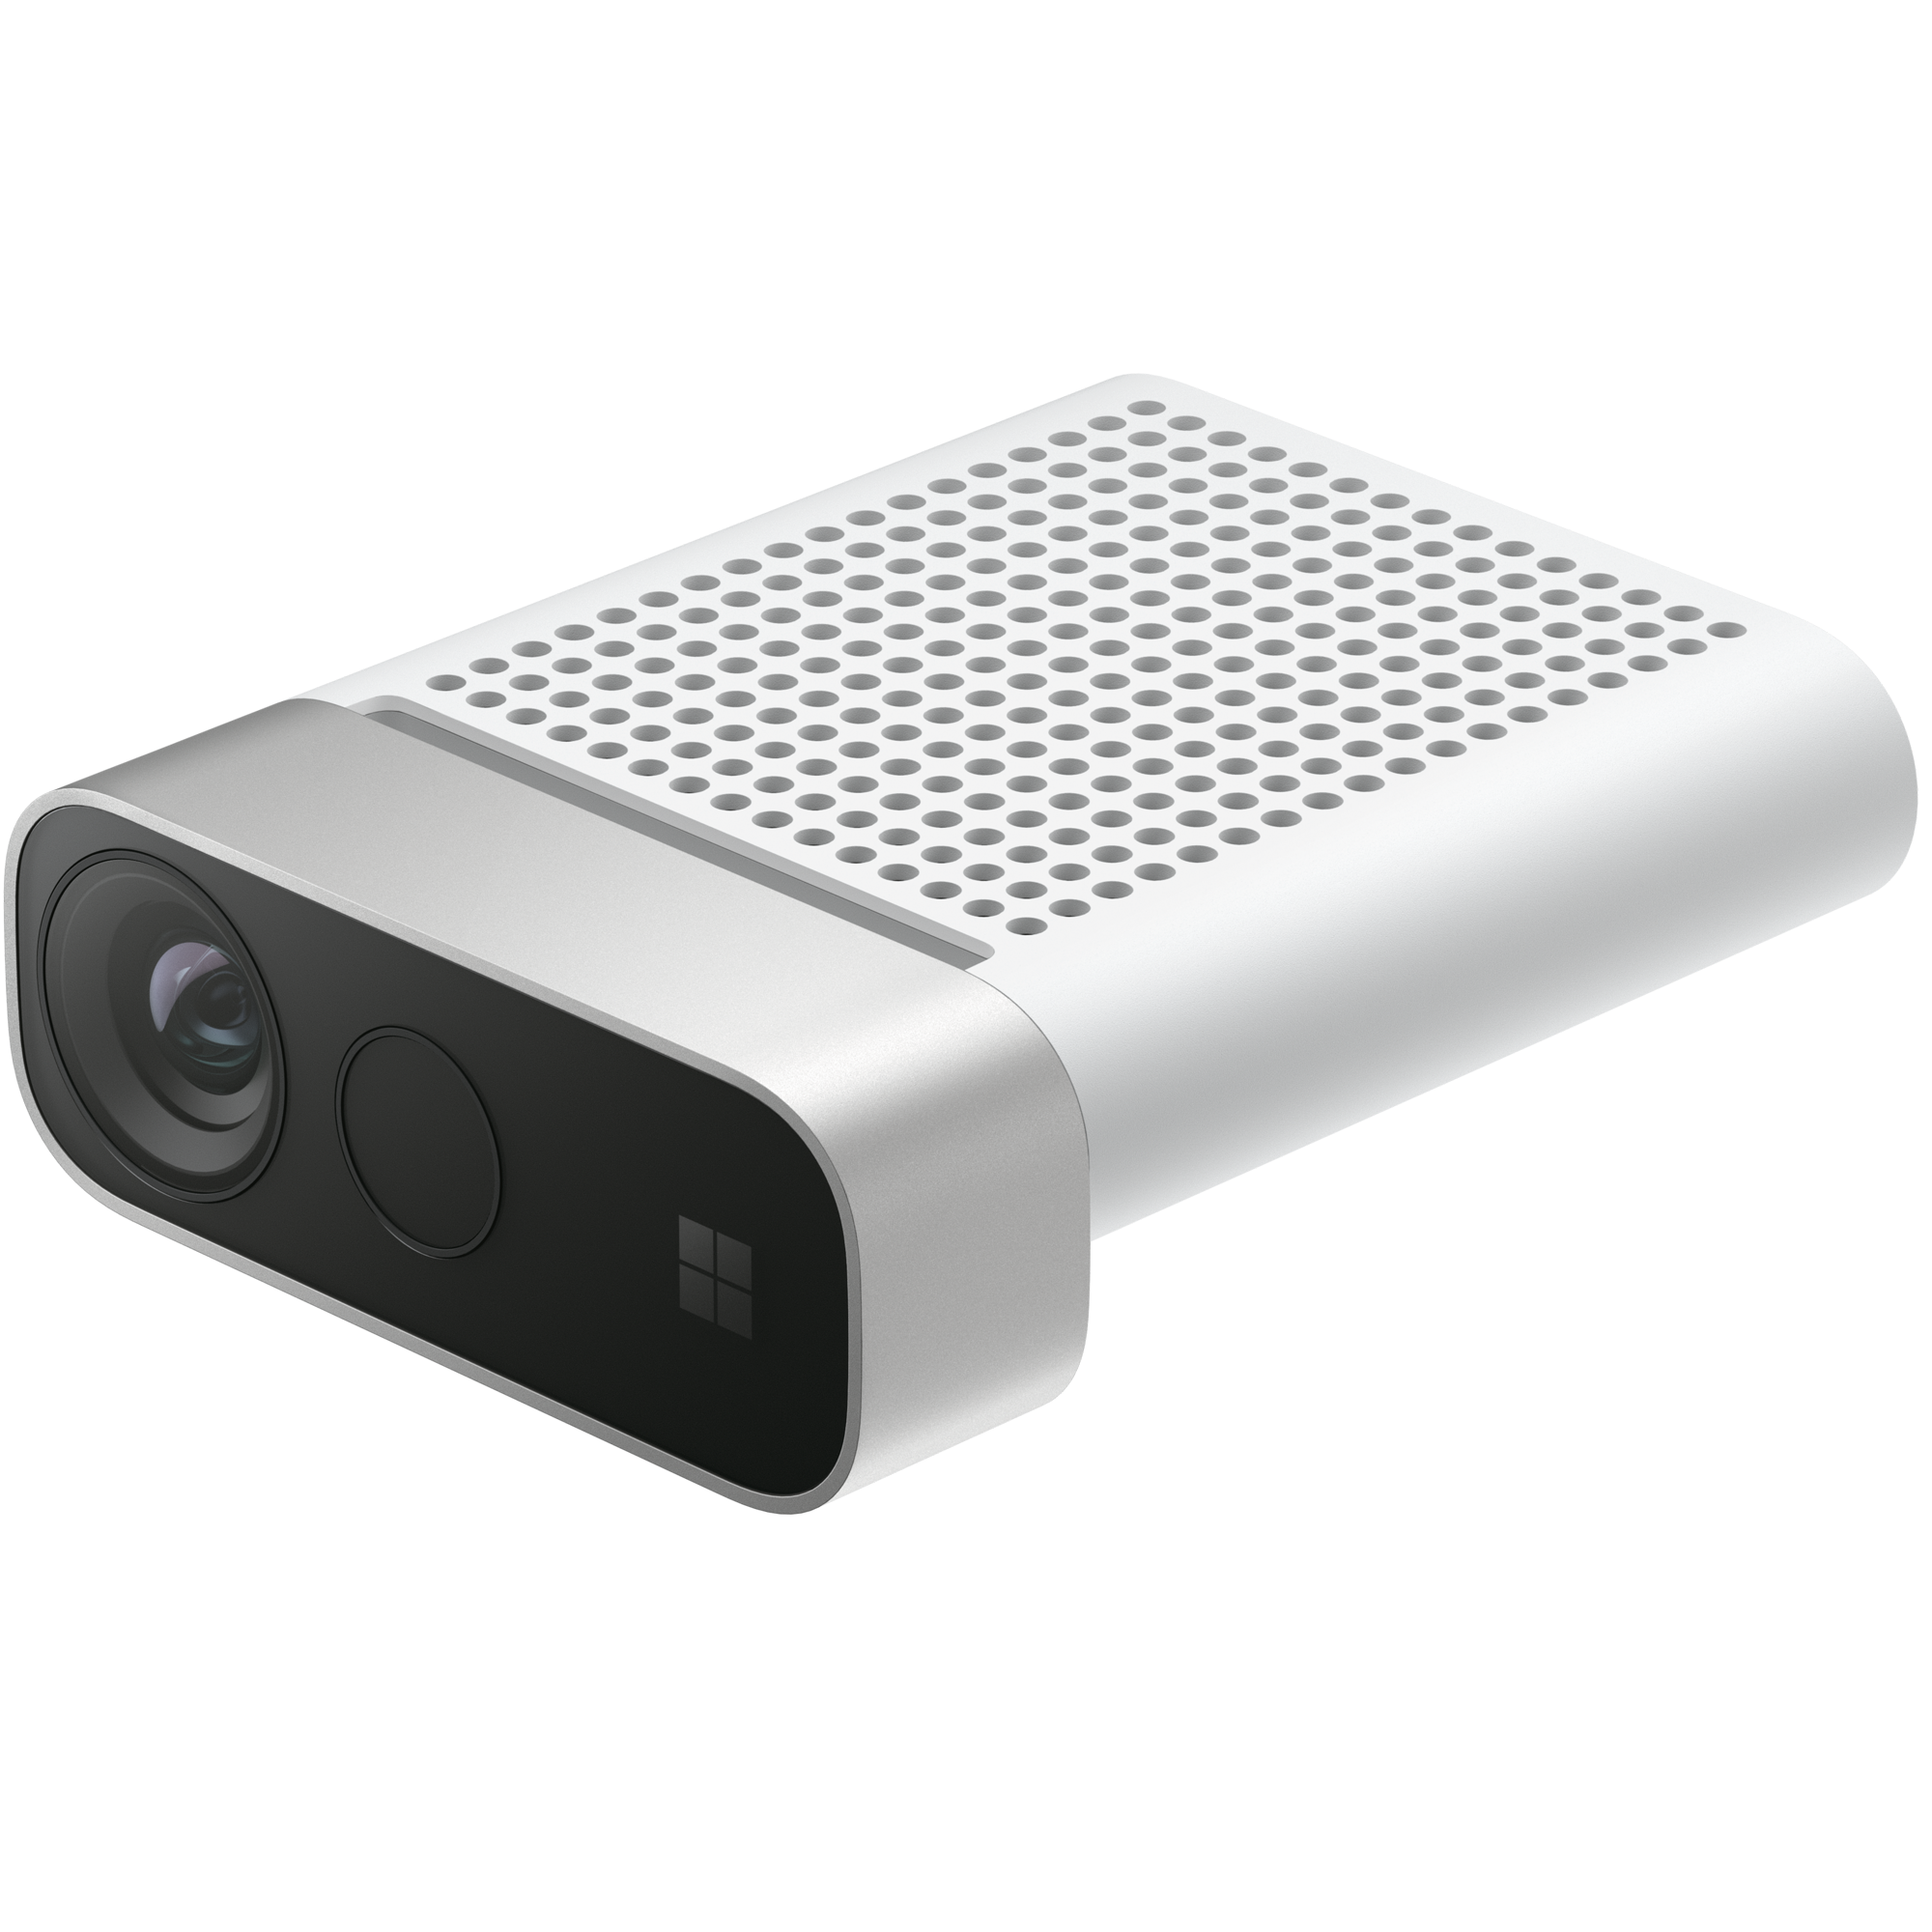
\includegraphics[width=8cm,height=5cm,]{./Images/azurekinect.png}
	\caption{Dispositivo Azure Kinect de Microsoft}
	\label{rehabexample}
\end{figure}

\subsection{PlayStation Camera desarrollado por Sony Computer Entertainment}

El modelo comercial actual es la PlayStation Camera, la cual es un sensor de movimiento y un accesorio de cara para la PlayStation 4 y la Play Station 5, fue desarrollado por Sony Computer Entertainment,.

Su modelo previo fue el PlayStation Eye, siendo lanzado al mercado desde el 2007, si bien fue lanzado al mercado antes que el Kinect, sus aplicaciones se distinguían en distintos campos y utilidades. Su visión estaba concentrada en una investigación\texttt{investigacion}  de chat audio visual con quien tengan conexión, además del reconocimiento facial, de gestos, colores y proporcionar con ello una realidad mixta para socializar.
\begin{figure}
	\centering
	\begin{subfigure}{.3\textwidth}
		\centering
		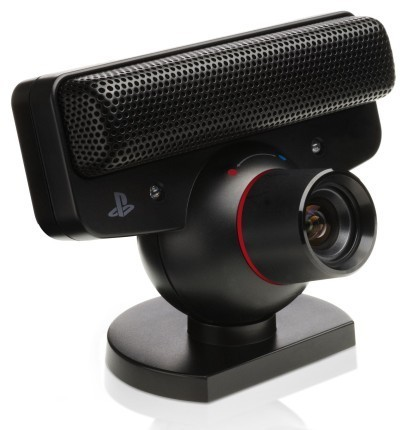
\includegraphics[width=5cm,height=5cm,]{./Images/eyeex.jpg}
		\caption{Dispositivo PS Eye}
		\label{eyeex}
	\end{subfigure}%
	\begin{subfigure}{.4\textwidth}
	\centering
	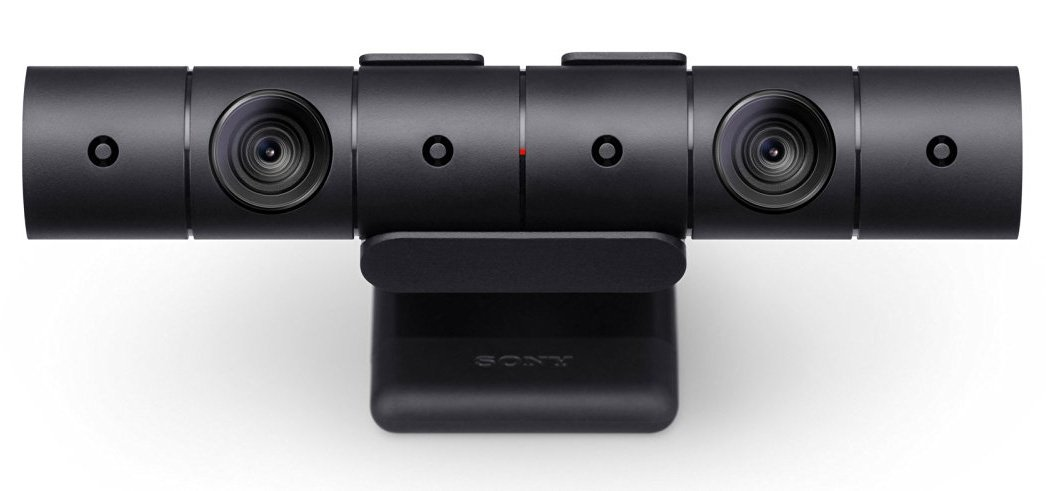
\includegraphics[width=7cm,height=4cm,]{./Images/cameraex.jpg}
	\caption{Dispositivo PS Camera}
	\label{cameraex}
	\end{subfigure}%
	\begin{subfigure}{0.3\textwidth}
		\centering
		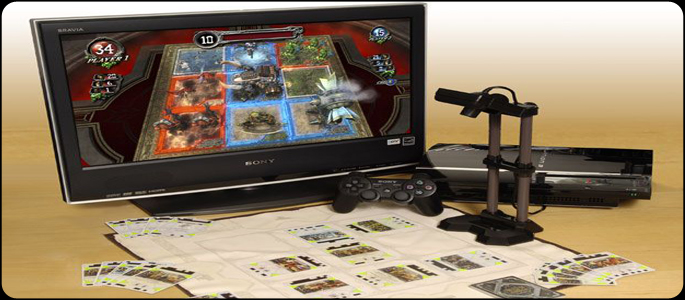
\includegraphics[width=6cm,height=4cm,]{./Images/eyeexuse.jpg}
		\caption{Ejemplo de Uso de PS Eye}
		\label{eyeexuse}
	\end{subfigure}
	\caption{Distintos Dispositivos Específicos para Body Tracking}
	\label{eyeExample}
\end{figure}

\subsection{Ámbito Clínico}
Realizando un enfoque principal en el papel de la rehabilitación, desde la perspectiva médica, se realizaron estudios sobre un uso alternativo a Body Tracking, distinguiendo su accesibilidad y fácil desarrollo, además que se reportan altos niveles de gozo con la interacción y ejercicio con familiares y amigos. 

Se realizaron múltiples estudios, para distintas enfermedades, lesiones y situaciones medicas, se mencionaran un par de ejemplos para señalar su eficiencia. Un grupo de investigadores, estudiaron el tratamiento de deficiencia neurológica empleando consolas, tales como el Sony Playstation®2 \cite{rand2008sony} y Nintendo Wii \cite{herz2013nintendo} como punto de apoyo para empleo en terapias, lo que niega la objetividad negativa hacia la iniciativa del empleo de sistemas interactivos de esta índole.\\

La detección de movimiento y la tecnología gráfica empleada en software comerciales no se limitan al movimiento de un control convencional, permiten al usuario sentir estímulos necesarios para optimizar las habilidades motoras precisas que se buscan rehabilitar, más allá de agitarse de un lado a otro. Como teoría no cumplen los requerimientos de intervención precisa de una manera sistemática, necesarios desde el punto de vista tradicional, sin embargo, su potencial puede ser útil en el camino de la rehabilitación \cite{lange2011markerless}. \\

Siendo un estudio en el ámbito, la rehabilitación basada en Simuladores Interactivos, creando desafíos de bajo costo y desarrollados de manera Amateur,  para secundar la motivación de personas hospitalizadas, particularmente aquellas que necesitan recuperarse de una lesión de trauma cerebral, médula espinal o amputaciones \cite{lange2011markerless}. 
\begin{figure}[t!]
	\centering
	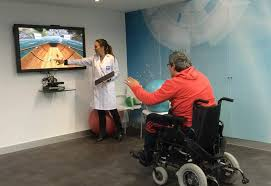
\includegraphics[width=8cm,height=5cm,]{./Images/rehabilitacionexample.jpg}
	\caption{Ejemplo de Rehabilitación empleando Body Tracking}
	\label{rehabexample}
\end{figure}
La retroalimentación indica que en general, se enmarcaron los desafíos como divertidos y retadores, viendo con positivismo su uso posterior en el hogar de estar disponible \cite{lange2011leveraging}.\\

\subsection{Ámbito Pedagógico}

Si bien se suspendieron las clases de este año académico a nivel primaria-secundaria en Bolivia, una obligación que consume una sustancial cantidad de tiempo es la asistencia escolar y una de las facetas importantes, la implementación de actividad física, conlleva un potencial impacto en la capacidad del estudiante de evadir una vida sedentaria reclusa y comprometerlo a actividades moderadamente intensas de practica fuera de la labor estudiantil \cite{daly2018systematic}.

Se realizaron estudios sobre el potencial de los sistemas interactivos y discusiones sobre la facilidad que proporcionan en la educación y enseñanza, sin embargo, el presupuesto necesario no es necesariamente bajo para un colegio, lo cual ha privado a Bolivia de considerar estas opciones. Si este caso no impusiera un impacto negativo en la decisión de implementarlos, podría ser considerado limpiamente como oportuno.\\

Los sistemas interactivos utilizan una tecnología basada en acciones de movimiento, el cual puede envolverse con un importante aspecto interactivo pedagógico, el beneficio a la inteligencia corporal-kinestésica. Se resalta el potencial que ofrece para mejorar la interacción y discusión saludable entre el alumnado y las habilidades de los profesores para manipular y presentar equipos y material multimedia. Como una herramienta educativa, tiene la capacidad de impulsar la motivación, promover el aprendizaje e interés de las actividades, crear un entorno agradable y competitivo en la clase\cite{pirie1995meaning}.\\

Sin embargo, no se puede descartar las dificultades del espacio requerido, la necesidad de calibrar los dispositivos y el cambio de metodología pedagógica para incluir el sistema interactivo, por encima de todo, la persuasión a las unidades estudiantiles y a los profesores de modificar la manera tradicional de enseñar educación física, ya que los estudios aún no son claros en su totalidad de que tan tangibles son los resultados en comparación al tradicional \cite{daly2018systematic}. \\
\begin{figure}[t!]
	\centering
	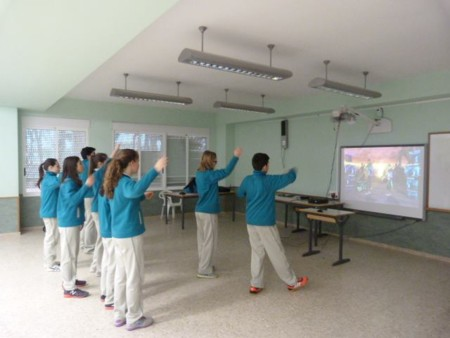
\includegraphics[width=8cm,height=5cm,]{./Images/kinectexampleschool.jpg}
	\caption{Ejemplo de Clase de Educación Física empleando Body Tracking}
	\label{claseEF}
\end{figure}

\subsection{Ámbito De Entretenimiento y Entrenamiento}

Un campo popular es aquel que requiere de una forma lúdica de realizar actividad física y ejercicio, ya que, al igual que en el ámbito pedagógico y clínico, su objetivo es incitar al usuario a realizar ejercicio de una u otra forma, sin embargo, esta vez el enfoque es distinto, buscando desgastar el cuerpo de los usuarios para poder relajarse o cansarse.

Este ámbito tiene una característica importante y es su amplio margen de usuarios potenciales, los cuales, han sido mermados debido a que hasta el momento, han tenido la necesidad de adquirir dispositivos como Kinect o Play Station Camera para acceder a estos juegos interactivos.

\subsubsection{Clasificación de Edades Para el Uso de Sistemas Interactivos de Entretenimiento y Entrenamiento}

Los sistemas interactivos están diseñados para distintos públicos según las temáticas que presenta el producto, en el caso de entretenimiento y entrenamiento, la población dirigida no tiene restricciones de edad, ya que títulos como Just Dance o Shape Up, ambas de la empresa Francesa Ubisoft, que clasifican sus títulos como apto para todo público en la clasificación por edades, exponiendo los sistemas de clasificación Europeo y Estadounidense, se encuentran el sistema PEGI y ESRB respectivamente.

En Latinoamericano, el año 2014, Colombia ofrece en la ley No. 1554, un nuevo sistema para clasificación de Sistemas Interactivos que se comercialicen de una u otra forma, como el alquiler o venta.
\begin{itemize}
	\item Circulación Abierta, la clasificación para el público general. En principio de temática deportiva, educativa, informativa y fantástico.
	\item Circulación Restringida, clasificada para un publico mayor a 18 años. Su contenido referencia actos discriminatorios, conflicto, consumo de sustancias controladas, consumo de bebidas alcohólicas, desnudez, sexo o sexualidad, lenguaje soez, derramamiento de sangre, muerte, lesiones humanas o apuestas por dinero o propiedades.
\end{itemize}

\subsubsection{Sistema PEGI}

En el sistema \href{https://pegi.info/es}{Pan European Game Information (PEGI)}, cuyo objetivo es clasificar el contenido de sistemas interactivos y software de entretenimiento. 
\\
El sistema PEGI fue desarrollado por la Federación Europea de Software Interactivo (ISFE) y se puso en practica desde el 9 de abril de 2003, empleado por 25 países. El sistema cuenta con la evaluación del Instituto Holandés para la Clasificación de Contenido Audiovisual (NICAM), como historial de trabajo, NICAM fue responsable también del sistema holandés para la clasificación de edades de películas.

\begin{figure}[t!]
	\centering
	
\includegraphics[width=9cm,height=4cm,]{./Images/pegi.png}
	\caption{Sistema De Clasificación PEGI}
	\label{pegi}
\end{figure}
Todas las categorías contienen un modo de juego en línea y de compras dentro del juego. En la figura \ref{pegi} se encuentran las categorías del sistema PEGI, los cuales son:
\begin{itemize}
	\item Apto para todo público: Violencia en un grado moderado.
	\item Apto para mayores de 7 años: Violencia moderada, uso de armas y terror moderado.
	\item Apto para mayores de 12 años: Violencia moderada, uso de armas, lesiones, muerte censurada, lenguaje soez, terror moderado, referencias vagas a sexo y apuestas moderadas y vigilancia.
	\item Apto para mayores de 16 años: Violencia, uso de armas, lesiones, muerte, derramamiento de sangre, lenguaje soez, terror, temas sexuales, sustancias controladas y apuestas.
	\item Solamente adultos: Además de todo lo anterior, se añade la discriminación y erotismo, solo para personas con criterio o conscientes.
\end{itemize}


\subsubsection{Sistema ESRB}

Con el mismo objetivo que el sistema PEGI, el sistema \href{https://www.esrb.org/}{Entertainment Software Rating Board (ESRB)}, es la versión estadounidense para clasificación de contenido de sistemas interactivos, para asignar categorías que dependen del contenido y temática. 
\\
Se estableció en 1994 por la Entertainment Software Association (ESA), la cual es una asociación comercial de la industria de sistemas interactivos en Estados Unidos. Se fundo inicialmente con el nombre de Interactive Digital Software Association (IDSA), renombrado el 16 de julio de 2003. Es conocido mundialmente por ser empleado por empresas que son miembros de ESA, entre ellos Capcom, Square Enix, Ubisoft, Bandai Namco Entertainment, Nintendo. 

La ESA también prepara la exposición anual de videojuegos Electronic Entertainment Expo (E3) en California, Los Ángeles.

\begin{figure}[t!]
	\centering
	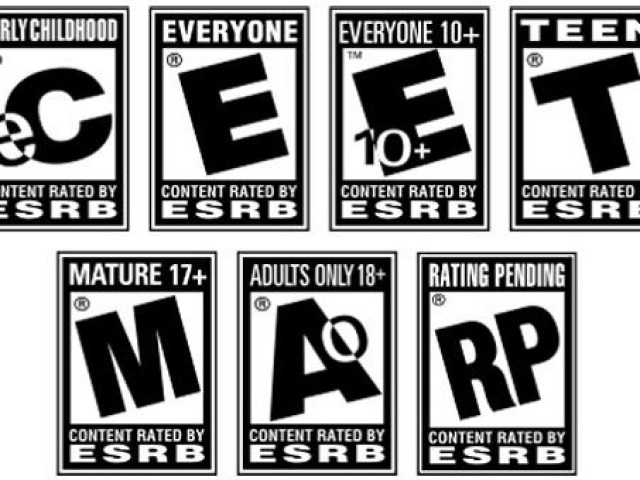
\includegraphics[width=10cm,height=5cm,]{./Images/esrb.jpg}
	\caption{Sistema De Clasificación ESRB}
	\label{esrb}
\end{figure}

En la figura \ref{esrb} se encuentran las categorías del sistema ESRB, los cuales son:
\begin{itemize}
	\item Early Childhood: Contenido apto para niños, específicamente desarrollados para publico infantil. Se retiro la categoría en 2018.
	\item Everyone: Una selección de títulos diseñados para todo publico, minimizando violencia fantástica y empleo de insultos leves. Aplica al deporte.
	\item Everyone 10 and up/Everyone: Permite violencia leve o fantastica, sangre animada, insultos leves. Apto para mayores de 10 años.
	\item Teen: Contiene derramamiento de sangre, temas sugerentes, violencia moderada o humor negro, en varios casos, juegos de azar o apuestas.
	\item Mature 17+: Contienen violencia, sangre, horror, temas sexuales e insultos. Apto para mayores de 17 años.
	\item Adults Only 18+: Escenas prolongadas de violencia o temas sexuales, apuestas y azar con dinero real o ficticio y sangre o desnudez frecuentes. Usualmente contiene temas de controversia o exageraciones que requieren de restricciones.
	\item Rating Pending: Se desconoce su categoría, debido a su reciente lanzamiento, usualmente depende de la intensidad de la temática presentada por el sistema interactivo.
\end{itemize}

